

\begin{figure*}[t]
\centering
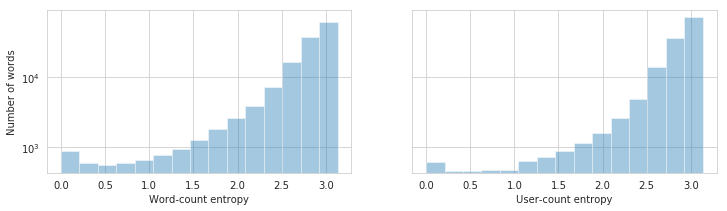
\includegraphics[width=\textwidth]{./images/entropies.png}
\caption{Histogram of word occurrence entropy ($H_w$). As one would expect, most words are used uniformly across the country} 
\label{fig:word_ocurrence_entropy} 
\end{figure*}


We can think of a \emph{regionalism} as a word whose use is not uniform across all the studied region, whose concentration is high in a specific part of the country. We are trying, in fact, to measure disorder of the use of a word, and there exists an information-theoretic tool for this: entropy.

It is known that entropy holds information about the semantic role played by a word \cite{montemurro2002entropic, montemurro2010towards}. High-entropy words, given a text, are more likely to be pronouns, connectors and other non-informative words, whereas its low-entropy counterparts are usually nouns and adjectives playing a key role in the document. 

Taking into account occurrence of words across a geographical region, words with high entropy (high disorder) can be regarded as words whose use is similar all across the region of study. On the other hand, low-entropy words are more used in a region than in the rest of it.

Let $p = (p_1, p_2, \ldots, p_N)$ the relative frequencies of occurrence of the word $\omega$ for each geographical region (in our case, provinces), the \emph{word-count entropy} is defined as:

\begin{equation}
    H_w(\omega) = -\sum \limits_{k=1}^{N} p_k \log(p_k)
\end{equation}


This measure does not take in account the frequency of words, which is also important. For instance, a word occurring once in a province has the same entropy as a word occurring millions of times at the same place. To remediate this issue, a measure based on \cite{montemurro2010towards} was developed, taking into account the frequency of use. We define the \emph{Information Value} of $w$ as:

\begin{equation}
  \label{eqn:iv_words}
  I_w(\omega) = p(\omega) \,  (\log(n) - H_w(\omega))
\end{equation}

The $log(n)$ in the formula represents the maximum possible value of $H(\omega)$ \cite{shannon2001mathematical}; for our work, recall that $n = 23$ (number of provinces in Argentina).

Another factor of information of a word is the amount of people using it on Twitter, something already used in previous works\cite{Cui:2012:DBE:2396761.2398519}. Using the same arguments as above, if $\omega$ is a word, and if $q_1, q_2, \ldots , q_n$ are the relative probabilities of a user of $\omega$ belonging to each province, we define the \emph{user-count entropy} as.

\begin{equation}
    H_p(\omega) = -\sum \limits_{k=1}^{N} q_k \log(q_k)
\end{equation}


Then, we define \emph{User-Count Information Value} of  $\omega$ as:

\begin{equation}
  \label{eqn:iv_users}
  I_p(\omega) = p(\omega) \, (\log(n) - H_p(\omega))
\end{equation}

This measures the concentration of the people using this word.  In \ref{fig:word_ocurrence_entropy} we can observe the distribution of \emph{Word-Count Entropy} and \emph{User-Count Entropy} for the words in our vocabulary. As one would expect, most words are used uniformly across the country —both in occurrences and in users of it.

To take into account both \emph{word-counts} and \emph{user-counts} we define a third measure called \emph{Mixed Information Value} as:

\begin{equation}
  I(\omega) = I_w(\omega)  I_p(\omega)
\end{equation}


High values of $I(w)$ are reached when information value on users and on ocurrences is also high.



Due to the Zipfian nature of the distribution of words, the frequency of use of the most-used words is many orders of magnitude higher than others. This phenomenon also occurs with the user count. So the $p(w)$ term in equations \eqref{eqn:iv_words} and \eqref{eqn:iv_users} becomes a problem as very frequent words would overcome their low entropy. To alleviate this, we performed a normalization on the word frequency as follows: let 

\begin{equation}
    M_w = \argmax\limits_{\omega \in W} \#\omega 
\end{equation}

we define then

\begin{equation}
    n_w(\omega) = \frac{\log(\# w)}{\log(M_w)}
\end{equation}

Due to the logarithm in the formula, terms with a high amount of occurrences have little difference of $n_w(\omega)$ between them.

In an analogous form, we define a normalization for the amount of people using a word, named $n_p$. Hence, we redefine our information measures as:

\begin{align}
  I_w(\omega) &= n_w(\omega) (\log(n) - H_w(\omega)) \\
  I_p(\omega) &= n_p(\omega) (\log(n) - H_p(\omega)) 
\end{align}


